% Generated by Sphinx.
\def\sphinxdocclass{report}
\documentclass[letterpaper,10pt,english]{sphinxmanual}
\usepackage[utf8]{inputenc}
\DeclareUnicodeCharacter{00A0}{\nobreakspace}
\usepackage[T1]{fontenc}
\usepackage{babel}
\usepackage{times}
\usepackage[Bjarne]{fncychap}
\usepackage{longtable}
\usepackage{sphinx}
\usepackage{multirow}


\title{Pychron Documentation}
\date{April 16, 2012}
\release{1.4}
\author{Jake Ross}
\newcommand{\sphinxlogo}{}
\renewcommand{\releasename}{Release}
\makeindex

\makeatletter
\def\PYG@reset{\let\PYG@it=\relax \let\PYG@bf=\relax%
    \let\PYG@ul=\relax \let\PYG@tc=\relax%
    \let\PYG@bc=\relax \let\PYG@ff=\relax}
\def\PYG@tok#1{\csname PYG@tok@#1\endcsname}
\def\PYG@toks#1+{\ifx\relax#1\empty\else%
    \PYG@tok{#1}\expandafter\PYG@toks\fi}
\def\PYG@do#1{\PYG@bc{\PYG@tc{\PYG@ul{%
    \PYG@it{\PYG@bf{\PYG@ff{#1}}}}}}}
\def\PYG#1#2{\PYG@reset\PYG@toks#1+\relax+\PYG@do{#2}}

\def\PYG@tok@gd{\def\PYG@tc##1{\textcolor[rgb]{0.63,0.00,0.00}{##1}}}
\def\PYG@tok@gu{\let\PYG@bf=\textbf\def\PYG@tc##1{\textcolor[rgb]{0.50,0.00,0.50}{##1}}}
\def\PYG@tok@gt{\def\PYG@tc##1{\textcolor[rgb]{0.00,0.25,0.82}{##1}}}
\def\PYG@tok@gs{\let\PYG@bf=\textbf}
\def\PYG@tok@gr{\def\PYG@tc##1{\textcolor[rgb]{1.00,0.00,0.00}{##1}}}
\def\PYG@tok@cm{\let\PYG@it=\textit\def\PYG@tc##1{\textcolor[rgb]{0.25,0.50,0.56}{##1}}}
\def\PYG@tok@vg{\def\PYG@tc##1{\textcolor[rgb]{0.73,0.38,0.84}{##1}}}
\def\PYG@tok@m{\def\PYG@tc##1{\textcolor[rgb]{0.13,0.50,0.31}{##1}}}
\def\PYG@tok@mh{\def\PYG@tc##1{\textcolor[rgb]{0.13,0.50,0.31}{##1}}}
\def\PYG@tok@cs{\def\PYG@tc##1{\textcolor[rgb]{0.25,0.50,0.56}{##1}}\def\PYG@bc##1{\colorbox[rgb]{1.00,0.94,0.94}{##1}}}
\def\PYG@tok@ge{\let\PYG@it=\textit}
\def\PYG@tok@vc{\def\PYG@tc##1{\textcolor[rgb]{0.73,0.38,0.84}{##1}}}
\def\PYG@tok@il{\def\PYG@tc##1{\textcolor[rgb]{0.13,0.50,0.31}{##1}}}
\def\PYG@tok@go{\def\PYG@tc##1{\textcolor[rgb]{0.19,0.19,0.19}{##1}}}
\def\PYG@tok@cp{\def\PYG@tc##1{\textcolor[rgb]{0.00,0.44,0.13}{##1}}}
\def\PYG@tok@gi{\def\PYG@tc##1{\textcolor[rgb]{0.00,0.63,0.00}{##1}}}
\def\PYG@tok@gh{\let\PYG@bf=\textbf\def\PYG@tc##1{\textcolor[rgb]{0.00,0.00,0.50}{##1}}}
\def\PYG@tok@ni{\let\PYG@bf=\textbf\def\PYG@tc##1{\textcolor[rgb]{0.84,0.33,0.22}{##1}}}
\def\PYG@tok@nl{\let\PYG@bf=\textbf\def\PYG@tc##1{\textcolor[rgb]{0.00,0.13,0.44}{##1}}}
\def\PYG@tok@nn{\let\PYG@bf=\textbf\def\PYG@tc##1{\textcolor[rgb]{0.05,0.52,0.71}{##1}}}
\def\PYG@tok@no{\def\PYG@tc##1{\textcolor[rgb]{0.38,0.68,0.84}{##1}}}
\def\PYG@tok@na{\def\PYG@tc##1{\textcolor[rgb]{0.25,0.44,0.63}{##1}}}
\def\PYG@tok@nb{\def\PYG@tc##1{\textcolor[rgb]{0.00,0.44,0.13}{##1}}}
\def\PYG@tok@nc{\let\PYG@bf=\textbf\def\PYG@tc##1{\textcolor[rgb]{0.05,0.52,0.71}{##1}}}
\def\PYG@tok@nd{\let\PYG@bf=\textbf\def\PYG@tc##1{\textcolor[rgb]{0.33,0.33,0.33}{##1}}}
\def\PYG@tok@ne{\def\PYG@tc##1{\textcolor[rgb]{0.00,0.44,0.13}{##1}}}
\def\PYG@tok@nf{\def\PYG@tc##1{\textcolor[rgb]{0.02,0.16,0.49}{##1}}}
\def\PYG@tok@si{\let\PYG@it=\textit\def\PYG@tc##1{\textcolor[rgb]{0.44,0.63,0.82}{##1}}}
\def\PYG@tok@s2{\def\PYG@tc##1{\textcolor[rgb]{0.25,0.44,0.63}{##1}}}
\def\PYG@tok@vi{\def\PYG@tc##1{\textcolor[rgb]{0.73,0.38,0.84}{##1}}}
\def\PYG@tok@nt{\let\PYG@bf=\textbf\def\PYG@tc##1{\textcolor[rgb]{0.02,0.16,0.45}{##1}}}
\def\PYG@tok@nv{\def\PYG@tc##1{\textcolor[rgb]{0.73,0.38,0.84}{##1}}}
\def\PYG@tok@s1{\def\PYG@tc##1{\textcolor[rgb]{0.25,0.44,0.63}{##1}}}
\def\PYG@tok@gp{\let\PYG@bf=\textbf\def\PYG@tc##1{\textcolor[rgb]{0.78,0.36,0.04}{##1}}}
\def\PYG@tok@sh{\def\PYG@tc##1{\textcolor[rgb]{0.25,0.44,0.63}{##1}}}
\def\PYG@tok@ow{\let\PYG@bf=\textbf\def\PYG@tc##1{\textcolor[rgb]{0.00,0.44,0.13}{##1}}}
\def\PYG@tok@sx{\def\PYG@tc##1{\textcolor[rgb]{0.78,0.36,0.04}{##1}}}
\def\PYG@tok@bp{\def\PYG@tc##1{\textcolor[rgb]{0.00,0.44,0.13}{##1}}}
\def\PYG@tok@c1{\let\PYG@it=\textit\def\PYG@tc##1{\textcolor[rgb]{0.25,0.50,0.56}{##1}}}
\def\PYG@tok@kc{\let\PYG@bf=\textbf\def\PYG@tc##1{\textcolor[rgb]{0.00,0.44,0.13}{##1}}}
\def\PYG@tok@c{\let\PYG@it=\textit\def\PYG@tc##1{\textcolor[rgb]{0.25,0.50,0.56}{##1}}}
\def\PYG@tok@mf{\def\PYG@tc##1{\textcolor[rgb]{0.13,0.50,0.31}{##1}}}
\def\PYG@tok@err{\def\PYG@bc##1{\fcolorbox[rgb]{1.00,0.00,0.00}{1,1,1}{##1}}}
\def\PYG@tok@kd{\let\PYG@bf=\textbf\def\PYG@tc##1{\textcolor[rgb]{0.00,0.44,0.13}{##1}}}
\def\PYG@tok@ss{\def\PYG@tc##1{\textcolor[rgb]{0.32,0.47,0.09}{##1}}}
\def\PYG@tok@sr{\def\PYG@tc##1{\textcolor[rgb]{0.14,0.33,0.53}{##1}}}
\def\PYG@tok@mo{\def\PYG@tc##1{\textcolor[rgb]{0.13,0.50,0.31}{##1}}}
\def\PYG@tok@mi{\def\PYG@tc##1{\textcolor[rgb]{0.13,0.50,0.31}{##1}}}
\def\PYG@tok@kn{\let\PYG@bf=\textbf\def\PYG@tc##1{\textcolor[rgb]{0.00,0.44,0.13}{##1}}}
\def\PYG@tok@o{\def\PYG@tc##1{\textcolor[rgb]{0.40,0.40,0.40}{##1}}}
\def\PYG@tok@kr{\let\PYG@bf=\textbf\def\PYG@tc##1{\textcolor[rgb]{0.00,0.44,0.13}{##1}}}
\def\PYG@tok@s{\def\PYG@tc##1{\textcolor[rgb]{0.25,0.44,0.63}{##1}}}
\def\PYG@tok@kp{\def\PYG@tc##1{\textcolor[rgb]{0.00,0.44,0.13}{##1}}}
\def\PYG@tok@w{\def\PYG@tc##1{\textcolor[rgb]{0.73,0.73,0.73}{##1}}}
\def\PYG@tok@kt{\def\PYG@tc##1{\textcolor[rgb]{0.56,0.13,0.00}{##1}}}
\def\PYG@tok@sc{\def\PYG@tc##1{\textcolor[rgb]{0.25,0.44,0.63}{##1}}}
\def\PYG@tok@sb{\def\PYG@tc##1{\textcolor[rgb]{0.25,0.44,0.63}{##1}}}
\def\PYG@tok@k{\let\PYG@bf=\textbf\def\PYG@tc##1{\textcolor[rgb]{0.00,0.44,0.13}{##1}}}
\def\PYG@tok@se{\let\PYG@bf=\textbf\def\PYG@tc##1{\textcolor[rgb]{0.25,0.44,0.63}{##1}}}
\def\PYG@tok@sd{\let\PYG@it=\textit\def\PYG@tc##1{\textcolor[rgb]{0.25,0.44,0.63}{##1}}}

\def\PYGZbs{\char`\\}
\def\PYGZus{\char`\_}
\def\PYGZob{\char`\{}
\def\PYGZcb{\char`\}}
\def\PYGZca{\char`\^}
\def\PYGZsh{\char`\#}
\def\PYGZpc{\char`\%}
\def\PYGZdl{\char`\$}
\def\PYGZti{\char`\~}
% for compatibility with earlier versions
\def\PYGZat{@}
\def\PYGZlb{[}
\def\PYGZrb{]}
\makeatother

\begin{document}

\maketitle
\tableofcontents
\phantomsection\label{index::doc}


Contents:


\chapter{Scripting}
\label{scripting::doc}\label{scripting:scripting}\label{scripting:welcome-to-pychron-s-documentation}

\section{General}
\label{general_scripting::doc}\label{general_scripting:general}
\begin{Verbatim}[commandchars=\\\{\}]
\PYG{c}{\PYGZsh{}==========================================================}
\PYG{k}{def} \PYG{n+nf}{main}\PYG{p}{(}\PYG{p}{)}\PYG{p}{:}
    \PYG{n}{info}\PYG{p}{(}\PYG{l+s}{'}\PYG{l+s}{this is an info message}\PYG{l+s}{'}\PYG{p}{)}
    \PYG{n}{acquire}\PYG{p}{(}\PYG{l+s}{'}\PYG{l+s}{pipette}\PYG{l+s}{'}\PYG{p}{)}
    \PYG{n}{info}\PYG{p}{(}\PYG{l+s}{'}\PYG{l+s}{aquired resourece - pipette}\PYG{l+s}{'}\PYG{p}{)}
    \PYG{n}{sleep}\PYG{p}{(}\PYG{l+m+mi}{15}\PYG{p}{)}
    \PYG{n}{release}\PYG{p}{(}\PYG{l+s}{'}\PYG{l+s}{pipette}\PYG{l+s}{'}\PYG{p}{)}
    \PYG{n}{begin\PYGZus{}interval}\PYG{p}{(}\PYG{l+m+mi}{120}\PYG{p}{)}
    \PYG{c}{\PYGZsh{}do some stuff ...}
    \PYG{n}{complete\PYGZus{}interval}\PYG{p}{(}\PYG{p}{)} \PYG{c}{\PYGZsh{}wait until 120 seconds have passed}
\PYG{c}{\PYGZsh{}===============================================================}
\end{Verbatim}


\subsection{functions}
\label{general_scripting:functions}\index{info() (built-in function)}

\begin{fulllineitems}
\phantomsection\label{general_scripting:info}\pysiglinewithargsret{\bfcode{info}}{\emph{msg}}{}
add info \code{msg} to the log

\end{fulllineitems}

\index{acquire() (built-in function)}

\begin{fulllineitems}
\phantomsection\label{general_scripting:acquire}\pysiglinewithargsret{\bfcode{acquire}}{\emph{resource}}{}
reserve the \code{resource} for use. blocks other scripts from using \code{resource} until
{\hyperref[general_scripting:release]{\code{release()}}} is called.

\end{fulllineitems}

\index{release() (built-in function)}

\begin{fulllineitems}
\phantomsection\label{general_scripting:release}\pysiglinewithargsret{\bfcode{release}}{\emph{resource}}{}
release \code{resource} so other scripts can use it.

\end{fulllineitems}

\index{sleep() (built-in function)}

\begin{fulllineitems}
\phantomsection\label{general_scripting:sleep}\pysiglinewithargsret{\bfcode{sleep}}{\emph{seconds}}{}
sleep for \code{seconds}. if \code{seconds\textgreater{}5} a timer will appear. decimal seconds are allowed e.g \code{sleep(0.5)}

\end{fulllineitems}

\index{gosub() (built-in function)}

\begin{fulllineitems}
\phantomsection\label{general_scripting:gosub}\pysiglinewithargsret{\bfcode{gosub}}{\emph{path\_to\_script}}{}
execute a pyscript located at \code{path\_to\_script}. \code{path\_to\_script} is relative to the current
script. e.g \code{gosub(commonscripts/fuse.py)}. commonscripts must be a directory in the same
directory this script is saved in.

\end{fulllineitems}

\index{begin\_interval() (built-in function)}

\begin{fulllineitems}
\phantomsection\label{general_scripting:begin_interval}\pysiglinewithargsret{\bfcode{begin\_interval}}{\emph{timeout}}{}
start an interval. if \emph{timeout\textgreater{}5} a timer will appear.

\end{fulllineitems}

\index{complete\_interval() (built-in function)}

\begin{fulllineitems}
\phantomsection\label{general_scripting:complete_interval}\pysiglinewithargsret{\bfcode{complete\_interval}}{}{}
wait unit \code{timeout} has elapsed

\end{fulllineitems}



\section{Writing Bakeout Scripts}
\label{bakeout_scripting:writing-bakeout-scripts}\label{bakeout_scripting::doc}
Here's how to write a bakeoutscript
\begin{enumerate}
\item {} 
launch BakeoutManager (Bo on the dock)

\item {} 
open the script editor (\code{Edit scripts} button). An empty script is opened as a default

\item {} 
use \code{Open} to open an existing script or just start writing one from scratch

\item {} 
write your script. see below

\item {} 
you may check the syntax of your script at any point by hitting \code{Test}. A dialog will pop up saying if there was a problem and what it was or if the script passed with no errors. The scripts syntax is also automatically checked before saving.

\item {} 
Use \code{Save} and \code{Save As} in the normal manner. script files should end with \textbf{.py} .  if the file ending is omitted a \textbf{.py} is appended automatically

\item {} 
close the script editor

\end{enumerate}

here is an example script

\begin{Verbatim}[commandchars=\\\{\}]
\PYG{c}{\PYGZsh{}===========================================================================}
\PYG{c}{\PYGZsh{}this is a comment in the script. use it at your leisure}
\PYG{c}{\PYGZsh{}the following line def main(): is required and the entry point for the script}
\PYG{k}{def} \PYG{n+nf}{main}\PYG{p}{(}\PYG{p}{)}\PYG{p}{:}
    \PYG{c}{\PYGZsh{}this is the body of the main function}
    \PYG{c}{\PYGZsh{}it should be one tab in}
    \PYG{n}{ramp}\PYG{p}{(}\PYG{l+m+mi}{150}\PYG{p}{,}\PYG{l+m+mi}{100}\PYG{p}{,}\PYG{n}{start}\PYG{o}{=}\PYG{l+m+mi}{45}\PYG{p}{)}  \PYG{c}{\PYGZsh{} comments can go on the same line as functions}
    \PYG{n}{setpoint}\PYG{p}{(}\PYG{l+m+mi}{150}\PYG{p}{,}\PYG{l+m+mi}{4}\PYG{p}{)}
    \PYG{n}{ramp}\PYG{p}{(}\PYG{l+m+mi}{0}\PYG{p}{,}\PYG{o}{-}\PYG{l+m+mi}{150}\PYG{p}{)}
\PYG{c}{\PYGZsh{}end of script}
\PYG{c}{\PYGZsh{}===========================================================================}
\end{Verbatim}

Lets break it down line by line.
\begin{itemize}
\item {} 
A comment can be added anywhere using the \code{\#} character

\item {} 
\code{def main():} defines a required function called ``main'' that will be executed when the script is run. \textbf{The main  function is necessary} and is added to an empty script by default.

\item {} 
the function \code{ramp(150,100,start=45)}   sets the controller to 45 C, then increases the temperature setting to 150 C at a rate of 100 C/hr

\item {} 
the function \code{setpoint(150,4)} sets the controller to a temperature of 150 C and holds it for 4 hours

\item {} 
\code{ramp(0,-100)} decreases the temperature setting from the current temperature to 0 C at a rate of -100 C/hr.

\item {} 
Notice that the \code{start} parameter of the {\hyperref[bakeout_scripting:ramp]{\code{ramp()}}} function is optional. If omitted the controller's current temperature is used as the starting point

\end{itemize}

To activate a script for a given controller use the drop down menu located above the \emph{Duration} box

To execute the bakeout hit \code{Execute}. \code{Stop} to Stop.

\scalebox{0.500000}{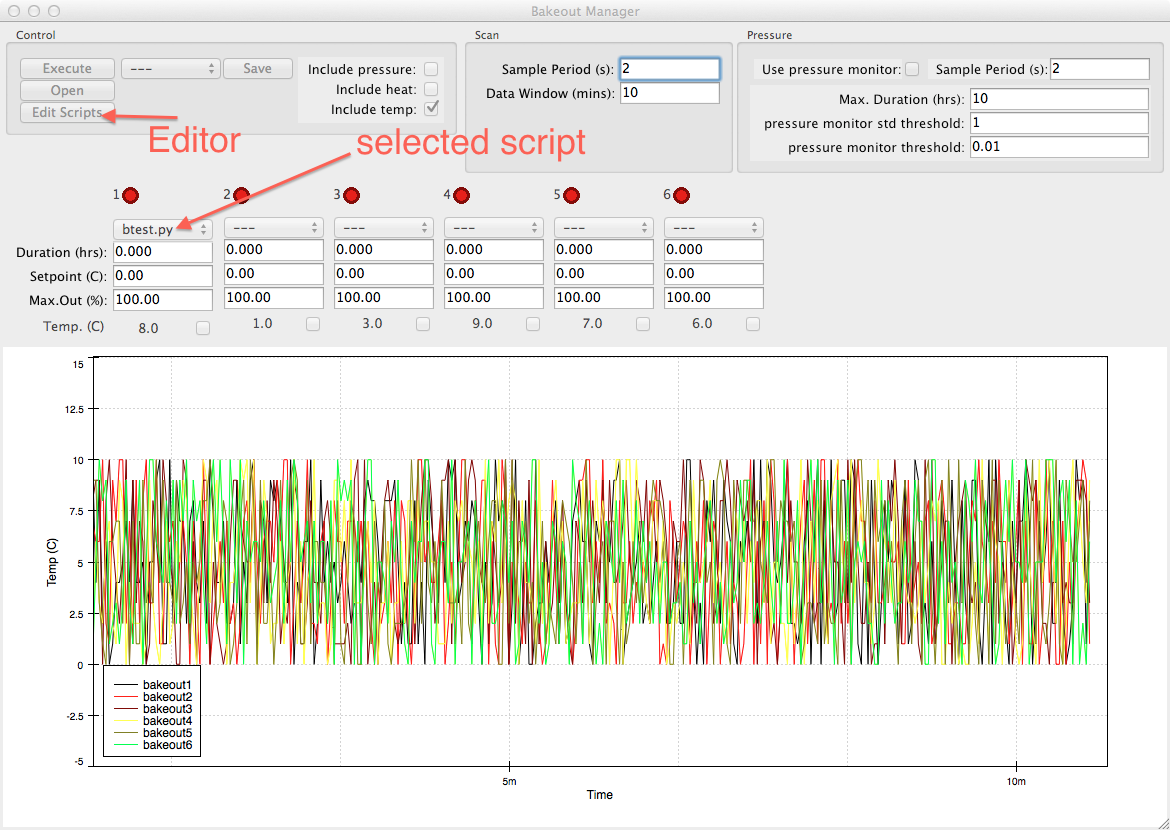
\includegraphics{bakeout_manager.png}}

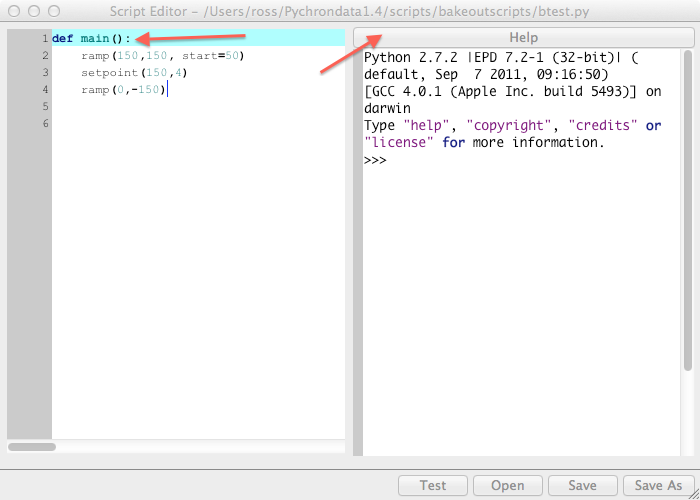
\includegraphics{bakeout_editor.png}


\subsection{bakeout functions}
\label{bakeout_scripting:bakeout-functions}\index{ramp() (built-in function)}

\begin{fulllineitems}
\phantomsection\label{bakeout_scripting:ramp}\pysiglinewithargsret{\bfcode{ramp}}{\emph{setpt}, \emph{rate}\optional{, \emph{start=None}, \emph{period=60}}}{}
ramp controller's setpoint from \code{start} to \code{setpt} at a rate of \code{rate} C\textbackslash{}hr.
if \code{start=None} then the controller's current \code{temperature} is used. \code{period} defines
seconds between setpoint updates. e.g. \code{period=30} sets the controllers setpoint every 30 seconds

\end{fulllineitems}

\index{setpoint() (built-in function)}

\begin{fulllineitems}
\phantomsection\label{bakeout_scripting:setpoint}\pysiglinewithargsret{\bfcode{setpoint}}{\emph{temperature}, \emph{duration}}{}
set controller's setpoint to \code{temperature} for \code{duration} hours

\end{fulllineitems}



\section{Writing Extraction Line Scripts}
\label{extraction_line_scripting:writing-extraction-line-scripts}\label{extraction_line_scripting::doc}
\begin{Verbatim}[commandchars=\\\{\}]
\PYG{k}{def} \PYG{n+nf}{main}\PYG{p}{(}\PYG{p}{)}\PYG{p}{:}
    \PYG{n+nb}{open}\PYG{p}{(}\PYG{l+s}{'}\PYG{l+s}{A}\PYG{l+s}{'}\PYG{p}{)}
    \PYG{n}{sleep}\PYG{p}{(}\PYG{l+m+mi}{1}\PYG{p}{)}
    \PYG{n}{close}\PYG{p}{(}\PYG{l+s}{'}\PYG{l+s}{A}\PYG{l+s}{'}\PYG{p}{)}

    \PYG{n}{info}\PYG{p}{(}\PYG{l+s}{'}\PYG{l+s}{this is an info message}\PYG{l+s}{'}\PYG{p}{)}

    \PYG{n}{acquire}\PYG{p}{(}\PYG{l+s}{'}\PYG{l+s}{pipette}\PYG{l+s}{'}\PYG{p}{)}
    \PYG{n}{info}\PYG{p}{(}\PYG{l+s}{'}\PYG{l+s}{loading air shot}\PYG{l+s}{'}\PYG{p}{)}
    \PYG{n+nb}{open}\PYG{p}{(}\PYG{l+s}{'}\PYG{l+s}{X}\PYG{l+s}{'}\PYG{p}{)}
    \PYG{n}{sleep}\PYG{p}{(}\PYG{l+m+mi}{15}\PYG{p}{)}
    \PYG{n}{close}\PYG{p}{(}\PYG{l+s}{'}\PYG{l+s}{X}\PYG{l+s}{'}\PYG{p}{)}
    \PYG{n}{release}\PYG{p}{(}\PYG{l+s}{'}\PYG{l+s}{pipette}\PYG{l+s}{'}\PYG{p}{)}
\end{Verbatim}


\subsection{extraction line functions}
\label{extraction_line_scripting:extraction-line-functions}\index{open() (built-in function)}

\begin{fulllineitems}
\phantomsection\label{extraction_line_scripting:open}\pysiglinewithargsret{\bfcode{open}}{\emph{alias}}{}
open the valve named \code{alias} e.g \code{open('A')}

\end{fulllineitems}

\index{close() (built-in function)}

\begin{fulllineitems}
\phantomsection\label{extraction_line_scripting:close}\pysiglinewithargsret{\bfcode{close}}{\emph{alias}}{}
open the valve named \code{alias} e.g \code{close('A')}

\end{fulllineitems}



\chapter{Procedures}
\label{procedures:procedures}\label{procedures::doc}

\section{CO$_{\text{2}}$ Stage Calibration}
\label{calibration::doc}\label{calibration:co2-stage-calibration}\begin{enumerate}
\item {} 
Move the laser to the center hole.

\item {} 
Select the correct stage map e.g \code{221-hole}

\item {} 
Select \code{pychron-auto} as the calibration style

\item {} 
Hit \code{Calibrate}

\end{enumerate}

Pychron will now automatically find up to five calibration holes. The calibration holes are
specified on the third line of the stage map file e.g \code{221-hole.txt}. The calibration holes
should be the N,E,S,W, and center holes.

Using the calibration holes Pychron calculates the center position and rotation of the tray.
With an accurate calibration, Pychron will then move to each hole and determine a corrected position.
This will take a few minutes.


\subsection{Autofocus}
\label{calibration:autofocus}
Pychron has an auto focus feature that can produce a very sharp image.
Configuration allows you to use various alogrithms to calculate the \emph{focus measure}
of an image. I find the Laplace filter with \textasciitilde{}50\% zoom produces a nice result.
Autofocus is actual a misnomer in this case. What is really happenig is called passive focus.
The \emph{focus measure} is calculated by applying a mathematical filter the the image. These filters
are used for example to calculate the gradient between adjacent pixels. Theoretically maximizing
the gradient yields the most focused image. For more information see
\href{http://en.wikipedia.org/wiki/Autofocus}{Autofocus}

Hit \code{Autofocus} to perform an autofocus routine


\section{Loading CO$_{\text{2}}$ Samples}
\label{co2_loading:loading-co2-samples}\label{co2_loading::doc}
!!Some please write me!!


\chapter{Remote Hardware}
\label{remote_hardware:remote-hardware}\label{remote_hardware::doc}
Remote hardware is used to allow other software clients access to pychron hardware, such as valves and laser systems.
A simple messaging system is used to pass information between pychron and a client. Currently the most
active client is Mass Spec which uses the remote hardware protocol to do all of its hardware tasks.

The protocol is broken in two sections {\hyperref[remote_hardware:system-calls-label]{\emph{System Calls}}} and {\hyperref[remote_hardware:laser-calls-label]{\emph{Laser Calls}}}.
Calls are simple ASCII text messages sent over the ethernet using either the \href{http://en.wikipedia.org/wiki/User\_Datagram\_Protocol}{UDP}
or \href{http://en.wikipedia.org/wiki/Transmission\_Control\_Protocol}{TCP} internet protocols

A response to a call is \code{OK}, a value, or an ErrorCode


\section{System Error Codes}
\label{system_errors::doc}\label{system_errors:system-error-codes}\phantomsection\label{system_errors:invalid-valve-error}

\begin{fulllineitems}
\pysigline{\bfcode{InvalidValveErrorCode}}
error code 001

\end{fulllineitems}



\section{Laser Error Codes}
\label{laser_errors:laser-error-codes}\label{laser_errors::doc}
InvalidValve


\section{System Calls}
\label{remote_hardware:system-calls-label}\label{remote_hardware:system-calls}

\begin{fulllineitems}
\pysigline{\bfcode{Open~alias}}
Open the valve called \code{alias}. {\hyperref[system_errors:invalid-valve-error]{\emph{InvalidValveErrorCode}}} return if \code{alias} not available

\end{fulllineitems}



\begin{fulllineitems}
\pysigline{\bfcode{Close~alias}}
Close the valve called \code{alias}. {\hyperref[system_errors:invalid-valve-error]{\emph{InvalidValveErrorCode}}} return if \code{alias} not available

\end{fulllineitems}



\begin{fulllineitems}
\pysigline{\bfcode{GetValveState~alias}}
Get \code{alias} state. Returns \code{0} for closed \code{1} for open

\end{fulllineitems}



\begin{fulllineitems}
\pysigline{\bfcode{GetValveStates}}
Get all the valves states as a word. Returns a string \textless{}alias\textgreater{}\textless{}state\textgreater{} e.g. \code{A1B0C1D1E0F0}

\end{fulllineitems}



\begin{fulllineitems}
\pysigline{\bfcode{GetValveLockStates}}
Get all the valves lock states as a word. Returns a string \textless{}alias\textgreater{}\textless{}lock\_state\textgreater{} e.g. \code{A1B0C1D1E0F0}

\end{fulllineitems}



\begin{fulllineitems}
\pysigline{\bfcode{StartMultRuns~multruns\_id}}
\end{fulllineitems}



\begin{fulllineitems}
\pysigline{\bfcode{CompleteMultRuns}}
\end{fulllineitems}



\begin{fulllineitems}
\pysigline{\bfcode{StartRun~runid}}
\end{fulllineitems}



\begin{fulllineitems}
\pysigline{\bfcode{CompleteRun}}
\end{fulllineitems}



\begin{fulllineitems}
\pysigline{\bfcode{PychronScript~script}}
\end{fulllineitems}



\begin{fulllineitems}
\pysigline{\bfcode{ScriptState}}
\end{fulllineitems}



\section{Laser Calls}
\label{remote_hardware:laser-calls-label}\label{remote_hardware:laser-calls}

\begin{fulllineitems}
\pysigline{\bfcode{Enable}}
Enable the laser.  This is required before the laser's power can be set using {\hyperref[remote_hardware:set-laser-power]{\emph{SetLaserPower}}}

\end{fulllineitems}



\begin{fulllineitems}
\pysigline{\bfcode{Disable}}
Disable the laser

\end{fulllineitems}

\phantomsection\label{remote_hardware:set-laser-power}

\begin{fulllineitems}
\pysigline{\bfcode{SetLaserPower~power}}
Set the laser's power to \code{power}. \code{power} must be between 0-100.

\end{fulllineitems}



\begin{fulllineitems}
\pysigline{\bfcode{ReadLaserPower}}
Read the lasers internal power meter. Returns an 8 bit value i.e 0-255

\end{fulllineitems}



\begin{fulllineitems}
\pysigline{\bfcode{GetLaserStatus}}
Return OK if the laser can be enabled. If an interlock is enabled, such as insufficient coolant flow, an error will be returned

\end{fulllineitems}



\begin{fulllineitems}
\pysigline{\bfcode{SetBeamDiameter}}
Set the beam diameter setting.

\end{fulllineitems}



\begin{fulllineitems}
\pysigline{\bfcode{GetBeamDiameter}}
Get the beam diameter setting.

\end{fulllineitems}



\begin{fulllineitems}
\pysigline{\bfcode{SetZoom~zoom}}
Set zoom. \code{zoom} must be between 0-100.

\end{fulllineitems}



\begin{fulllineitems}
\pysigline{\bfcode{GetZoom}}
Get zoom. returns value between 0-100.

\end{fulllineitems}



\begin{fulllineitems}
\pysigline{\bfcode{GetPosition}}
Returns a comma separated list of positions X,Y,Z

\end{fulllineitems}



\begin{fulllineitems}
\pysigline{\bfcode{GoToHole~holenum}}
Go to hole \code{holename}. InvalidHoleErrorCode returned if hole is not in the current stage map.

\end{fulllineitems}



\begin{fulllineitems}
\pysigline{\bfcode{GetJogProcedures}}
Return a list of available Jog procedures. Jog is a MassSpec term and a misnomer. Pychron internal refers
to them as Patterns.

\end{fulllineitems}



\begin{fulllineitems}
\pysigline{\bfcode{DoJog~name}}
Launch the jog named \code{name}.

\end{fulllineitems}



\begin{fulllineitems}
\pysigline{\bfcode{AbortJog}}
Abort the current jog

\end{fulllineitems}



\begin{fulllineitems}
\pysigline{\bfcode{SetX~xpos}}
Set the laser's stage controller X axis to \code{xpos}.

\end{fulllineitems}



\begin{fulllineitems}
\pysigline{\bfcode{SetY~ypos}}
Set the laser's stage controller X axis to \code{ypos}.

\end{fulllineitems}



\begin{fulllineitems}
\pysigline{\bfcode{SetZ~zpos}}
Set the laser's stage controller X axis to \code{zpos}.

\end{fulllineitems}



\begin{fulllineitems}
\pysigline{\bfcode{SetXY~xypos}}
Set the laser's stage controller X and Y axes to \code{xypos}. \code{xypos} should be a comma separated list of numbers.
e.g \code{SetXY 10.1,-5.03}

\end{fulllineitems}



\begin{fulllineitems}
\pysigline{\bfcode{GetXMoving}}
\end{fulllineitems}



\begin{fulllineitems}
\pysigline{\bfcode{GetYMoving}}
\end{fulllineitems}



\begin{fulllineitems}
\pysigline{\bfcode{GetDriveMoving}}
\end{fulllineitems}



\begin{fulllineitems}
\pysigline{\bfcode{StopDrive}}
\end{fulllineitems}



\begin{fulllineitems}
\pysigline{\bfcode{SetDriveHome}}
\end{fulllineitems}



\begin{fulllineitems}
\pysigline{\bfcode{SetHomeX}}
\end{fulllineitems}



\begin{fulllineitems}
\pysigline{\bfcode{SetHomeY}}
\end{fulllineitems}



\begin{fulllineitems}
\pysigline{\bfcode{SetHomeZ}}
\end{fulllineitems}



\chapter{Indices and tables}
\label{index:indices-and-tables}\begin{itemize}
\item {} 
\emph{genindex}

\item {} 
\emph{modindex}

\item {} 
\emph{search}

\end{itemize}



\renewcommand{\indexname}{Index}
\printindex
\end{document}
